\documentclass[11pt,a4paper]{article}
\usepackage[utf8]{inputenc}

\pagenumbering{arabic}
\usepackage[margin=1.0in]{geometry}
\usepackage{natbib} 
\usepackage{hyperref}
\usepackage{enumitem}
\usepackage{graphicx} % needed for \includegraphics
\usepackage{caption}

\newcommand{\todo}[1]{\textbf{\textcolor{red}{#1}}}
\newcommand{\MESA}{\texttt{MESA}\,}

% define a bunch of colors for pretty bash code blocks
\usepackage{xcolor}  % for coloring
\definecolor{bgdark}{rgb}{0.27,0.27,0.27}
\definecolor{lighttext}{rgb}{0.95,0.95,0.95}
\definecolor{bashgreen}{rgb}{0.5,1.0,0.5}
\definecolor{bashblue}{rgb}{0.5,0.8,1.0}
\definecolor{bashcomment}{rgb}{0.6,0.6,0.6}
\definecolor{bashstring}{rgb}{1.0,0.6,0.6}

% For pretty code blocks
\usepackage{listings}
% Bash style 
\lstset{
  language=bash,
  basicstyle=\ttfamily\small\color{lighttext},
  backgroundcolor=\color{bgdark},
  keywordstyle=\color{bashblue},
  commentstyle=\color{bashcomment},
  stringstyle=\color{bashstring},
  numbers=left,
  numberstyle=\tiny\color{bashcomment},
  stepnumber=1,
  frame=single,
  breaklines=true,
  showstringspaces=false
}
% Python style
\definecolor{pylightbg}{RGB}{250,250,250}
\definecolor{pyblue}{RGB}{0,0,180}      % keywords
\definecolor{pygreen}{RGB}{0,150,0}     % comments
\definecolor{pyred}{RGB}{180,0,0}       % strings
\definecolor{gray}{gray}{0.5}           % line numbers
\lstdefinestyle{pythonstyle}{
  language=Python,
  basicstyle=\ttfamily\small\color{black},
  backgroundcolor=\color{pylightbg},
  keywordstyle=\color{pyblue}\bfseries,
  commentstyle=\color{pygreen}\itshape,
  stringstyle=\color{pyred},
  numbers=left,
  numberstyle=\tiny\color{gray},
  stepnumber=1,
  frame=single,
  breaklines=true,
  showstringspaces=false
}


% For making the pro-tip boxes
\usepackage[most]{tcolorbox}
% define colors for the pro-tip boxes
\definecolor{protipbg}{HTML}{ebf0f2}    % 
\definecolor{protipborder}{HTML}{B0CAD4} % 
\definecolor{protiptext}{HTML}{003049}  % dark slate
\tcbset{
  protipbox/.style={
    colback=protipbg,
    colframe=protipborder,
    coltext=protiptext,
    fonttitle=\bfseries,
    title=Pro Tip,
    rounded corners,
    boxrule=0.pt,
    left=6pt,
    right=6pt,
    top=5pt,
    bottom=5pt
  }
}


%%%%%%%%%%%%%%%%%%%%%%%%%%%%%%%%%%%%%%%%%%%%
\begin{document}


\title{
    \textbf{\texttt{MESA} tutorial: Session 2} \\
    \textbf{\Large MESA output and Intermediate mass stars}
}
\date{}
\maketitle
\vspace{-1cm}


\noindent {\color{blue}Hand in your answers to all the numbered questions (i.e. 3.1 a, b, c etc.), they will make up your grade for the MESA practicum part of the course.}

%%%%%%%%%%%%%%%%%%%%%%%%%%%%%%%%%%%%%%%%%%%
\section{Understanding MESA output}

The following is a summary of the official \href{https://docs.mesastar.org/en/latest/using_mesa/output.html}{MESA documentation}. For a more comprehensive overview of available output options, please refer directly to the documentation.
%
You might have noticed that \MESA stores its output as plain text files in the \texttt{LOGS} directory. 
%
There are two main types of output:

\begin{itemize}
  \item \textbf{history.data:} logs each model's evolution in one line per model. The first line contains column indices, the second column names, and the remainder the data. Note: in case of a restart, older models are not removed—new data is appended. As a result \textit{the model\_numbers are not guaranteed to be monotonically increasing!} Existing tools (like \texttt{MESA Reader} below) automatically take care of this, but if you write your own parser, be aware of this.
  
  \item Each \textbf{profile**.data:} file contains a snapshot of a single model's structure. Each profile includes both global properties of the star, such as its age, and a large set of properties for each point in the model of the star given one line per point. In each case, the lines of data are preceded by a line with column numbers and a line with column names. 

\end{itemize}

\noindent Lastly, you might also notice a \textbf{profiles.index} file. This maps profile filenames to model numbers. MESA saves profiles only at selected steps. Each line lists a model number, its priority (1 or 2), and the corresponding profile number.


You can customize the \texttt{MESA} output through the \texttt{history\_columns.list} and \\
\texttt{profile\_columns.list} files. In order to customize the output, just copy these files to your work directory, and uncomment the variables you want to include in the output. You can find default variations of these files in the \texttt{\$MESA\_DIR/star/defaults/} directory. 
We will control some of the output of your \texttt{MESA} models in section \ref{sec:make_kippenhahn}.



%%%%%%%%%%%%%%%%%%%%%%%%%%%%%%%%%%%%%%%%
\paragraph{Using MESA Reader}
\texttt{MESA Reader} is a \texttt{Python} tool for reading and plotting history and profile data; see \href{https://docs.mesastar.org/en/latest/using_mesa/output.html#plotting-mesa-output}{MESA Reader} for details. Although \MESA outputs text files, restarts can duplicate model numbers and large headers make manual parsing tedious—\texttt{MESA Reader} handles all of this for you!

We want to install \texttt{MESA Reader}, but in such a way that we can always activate/access it, regardless of which computer we are using in the Faculty. 
Turns out that python \href{https://virtualenv.pypa.io/en/latest/user_guide.html}{\texttt{virtual environments}} are exactly what we are looking for!




%%%%%%%%%%%%%%%%%%%%%%%%%%%%%%%%%%%%%%%%%%%
\section{Jupyter Hub and virtual environments}

Throughout this course, we will use \texttt{Jupyter Notebooks} to analyse our results. 
If you have correctly copied your data to your home directory as explained in the previous session, you can access your this data via the RU JupyterHub: \url{https://jupyterhub.science.ru.nl/} and logging in with your science account.

You can create a Jupyter Notebook by clicking \texttt{File>New>Notebook}. It ask you which kernel to use: \texttt{Python3 ipykernel} will work out of the box for general analysis, but it does not have \texttt{MESA Reader} installed. For this purpose we will create our own \texttt{virtual environment} (venv) in which we install \texttt{MESA Reader} and other useful packages.



\paragraph{Creating a virtual environment}


\begin{itemize}

  \item When you are logged in, open a \textit{Jupyter Hub} terminal

\begin{figure}[h] % [h] = here, [t] = top, [b] = bottom, [p] = separate page
    \centering
    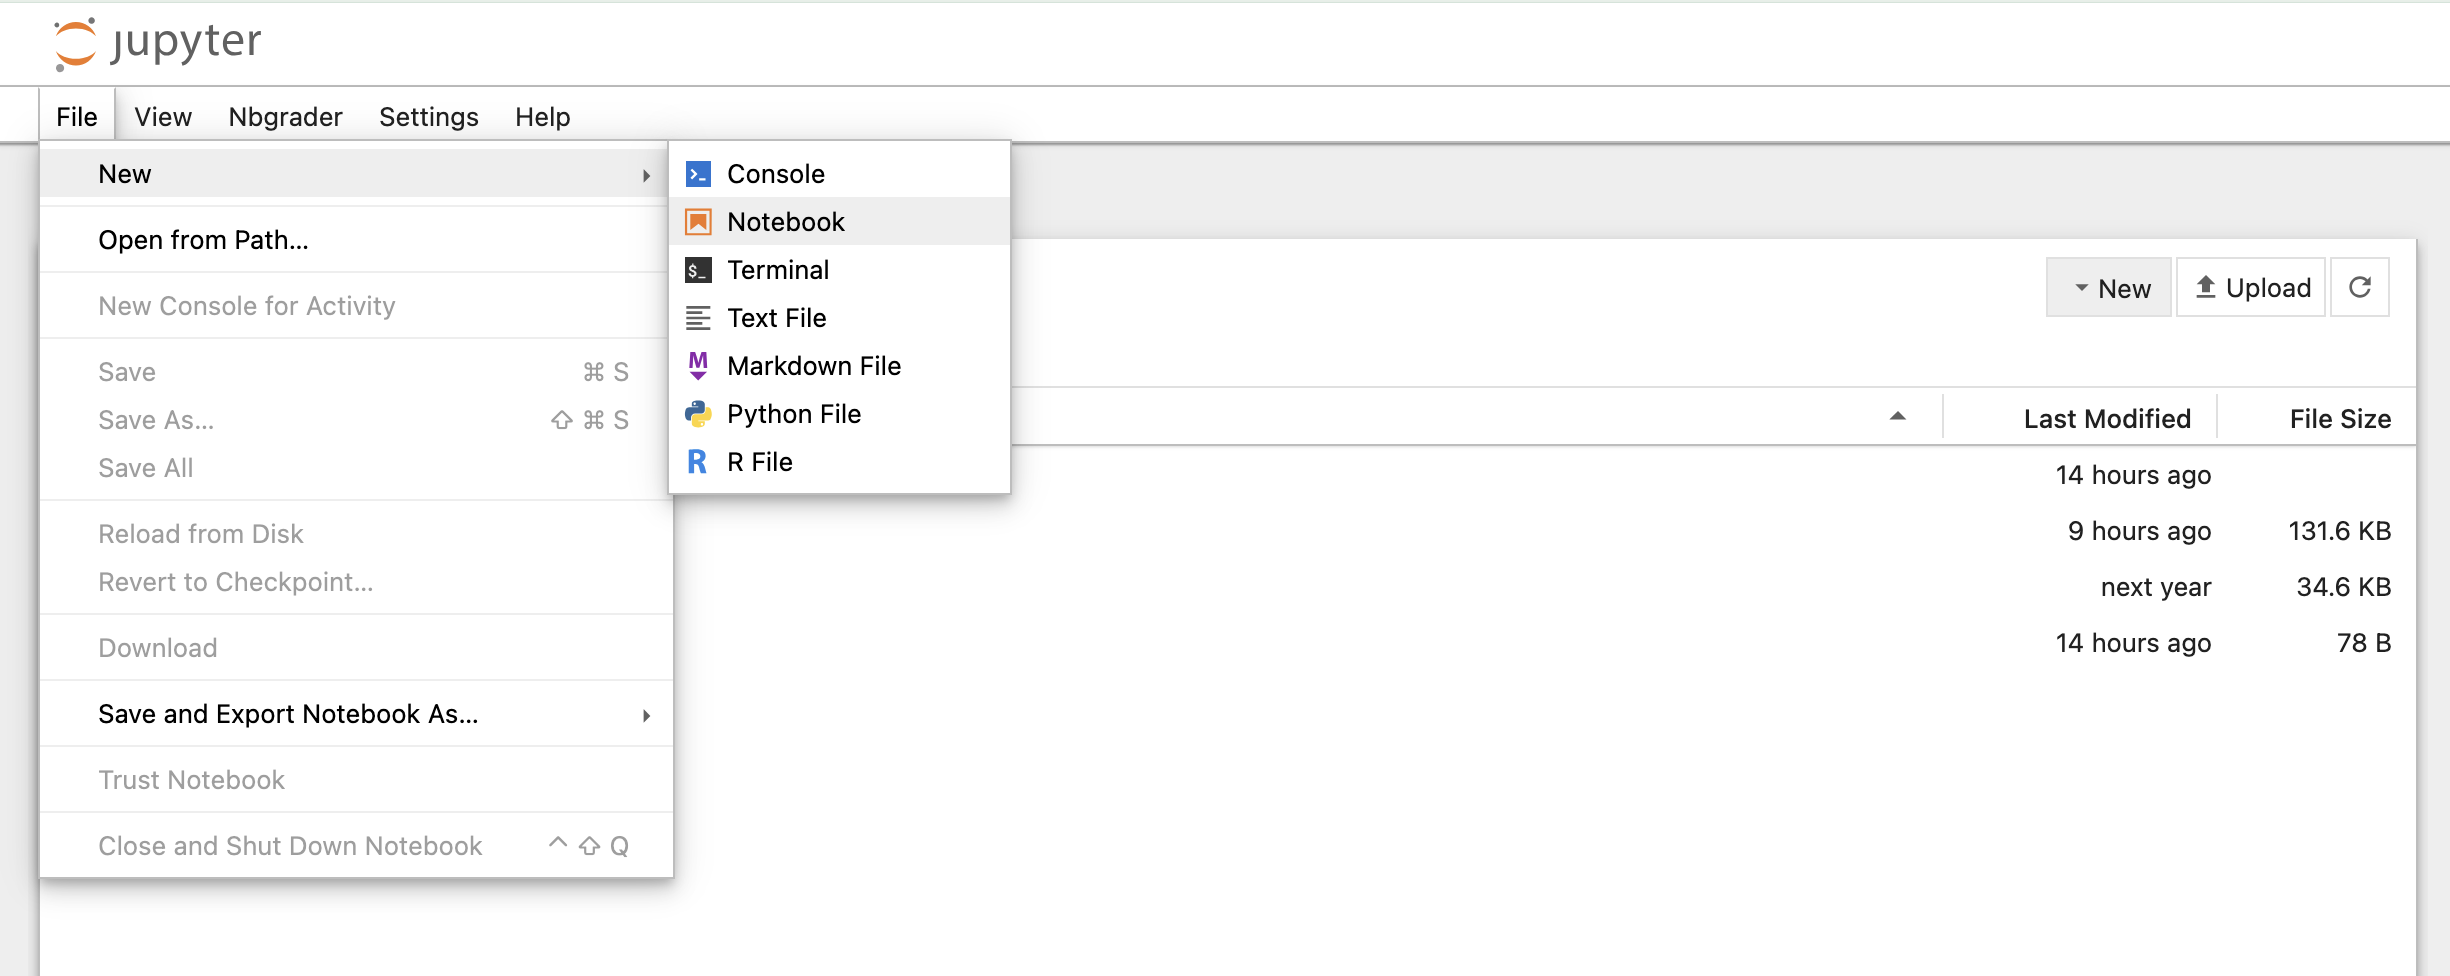
\includegraphics[width=\textwidth]{open_jupyternotebook.png} % path to your figure
    \caption*{ }
    \label{fig:myplot}
\end{figure}

  \item Inside your JupyterHub terminal, \textbf{Create a virtual environment} by running the following:
  \begin{lstlisting}
  mkdir -p ~/venvs     # make dir to store venvs
  cd ~/venvs           # go to that directory
  python -m venv myenv # create a venv called myenv
  source ~/venvs/myenv/bin/activate  # activate venv
  \end{lstlisting}

  You will notice that your terminal prompt changes adding \texttt{(myenv)} to the start, indicating that you are now working inside the virtual environment. To deactivate the virtual environment, simply run: \texttt{deactivate}.

  We need to ensure the package manager 'pip install' is up to date and available in our venv: 
  \begin{lstlisting}
  python -m ensurepip --upgrade
  python -m pip install --upgrade pip setuptools wheel ipykernel
  \end{lstlisting}


  \item While your venv is active, you can install Mesa Reader by running:
\begin{lstlisting}
  python -m pip install mesa-reader
\end{lstlisting}

    You can install all kinds of useful python packages like this in your venv using \texttt{python -m pip install <package\_name>}.\footnote{Note that normally you often use the slightly simpler \texttt{pip install <package\_name>}, but this can sometimes lead to some issues with the environment not being recognized due to PATH issues.}

    If for some reason you encounter trouble with the pip install, you can alternatively directly git clone (download) the code from the project's \href{https://github.com/wmwolf/py_mesa_reader}{Github repository} somewhere in your \texttt{home} directory (e.g. \verb|~/codes|)\footnote{\texttt{ \~  } is an alias for your home directory.} by running:
\begin{lstlisting}
  git clone https://github.com/wmwolf/py_mesa_reader.git ~/codes/py_mesa_reader
\end{lstlisting}
    Then run \texttt{python setup.py install} inside the cloned directory.


  Next, we need to register our venv as a Jupyter kernel:

\begin{lstlisting}
 pip install ipykernel     # makes venv able to run noteboooks
 python -m ipykernel install --user --name=myenv --display-name "Python (myenv)"
\end{lstlisting}

this should give you a message like: "Installed kernelspec myenv in ..."


  % Make sure your notebook is inside your plotting folder as to be able to access \texttt{MESA Reader}.}, or \texttt{Spyder3}\footnote{When running scripts in \texttt{Spyder}, you need to change the working directory as to have access to \texttt{MESA Reader} by going to \texttt{Run}, \texttt{Configuration per file...}, and changing \texttt{Working Directory settings} by putting in the correct path to your plotting folder with the \texttt{The following directory} option.}. To read in the data, you need to move the \texttt{history.data} files from your \texttt{scratch} directory to somewhere in your plotting folder, for example inside a folder called \texttt{data} and there inside a folder called after its run (e.g. \texttt{M3.0ov0}).
  % For this example, you use the following line in your \texttt{Python} script:
  
  \item Open a new notebook, you should now see your newly created \texttt{Python (myenv)} as an option in the kernel dropdown menu. Note that you can always switch kernels by clicking on the kernel name in the top right of your notebook.
  
  \item You should now be able to import \texttt{MESA Reader} without any errors, type:
  \begin{lstlisting}[style=pythonstyle]
  import mesa_reader as mr
  \end{lstlisting}

  and run your cell (\texttt{Shift + Enter})

  Note some other useful imports for calculating and plotting purposes could be:
  \begin{lstlisting}[style=pythonstyle]
    import numpy as np
    import matplotlib.pyplot as plt
    import astropy.units as u
    import astropy.constants as const
  \end{lstlisting}

  All of these packages can be installed in your venv using \texttt{pip install <package\_name>} in your jupyter terminal as explained above. We leave it to you to figure out which \texttt{pip install} commands do you need to run to get all the aforementioned packages. 

\end{itemize}

% \subsection*{Using \texttt{MesaLogDir}}

% \begin{verbatim}
% l = mr.MesaLogDir('./LOGS')

% # Load by model or profile number
% p_300 = l.profile_data(300)
% p_12 = l.profile_data(profile_number=12)

% # Load the most recent profile
% p_last = l.profile_data()
% \end{verbatim}


%%%%%%%%%%%%%%%%%%%%%%%%%%%%%%%%%%%%%%%%%%%
\section{Overshooting in an intermediate-mass star}

We will now investigate the effect of overshooting. In order to do this, we evolve an intermediate-mass star for different levels of convective overshooting.


\begin{enumerate}

\item[3.1] \textbf{Download and set up the work folder.} 
Instead of starting from the beginning and copying the model work directory like last time to edit, a \texttt{MESA} model has largely been constructed for you already. 

\begin{itemize}
    \item Download the tar file from Brightspace and unpack it. This can be done using the archive manager by extracting the contents to your desired location on the \texttt{scratch} disc, or using the terminal by typing \verb|tar -xvf session2.tar| in the directory where you downloaded the tar file and then moving the directory to your desired location on the \texttt{scratch} disc using a \texttt{cp -R} command. This file contains a \texttt{MESA} work folder in which we will work. 



    \item Once you open the \verb|inlist_project| file, you will find a number of controls available for the model. First, choose a mass for the star between 2.5 M$_\odot$ and 10 M$_\odot$, and modify the inlist accordingly. Note that the stopping condition allows the star to evolve up to the end of core helium burning. You may further notice several lines commented out concerning Convective overshooting. We will run several models for different values of the overshooting parameter. 

    \item First, compile (\verb|./mk|) and run (\verb|./rn|) the model without any overshooting. 
    Use the various \texttt{PGSTAR} windows to follow and understand the evolution of this star. One of the \texttt{PGSTAR} windows is a Kippenhahn diagram, which shows information about the structure of the star as it evolves. Also try to understand this plot.
    %\emph{Note:} You can zoom in and out on the time axis of the Kippenhahn plot by changing \verb|Kipp_max_width| in \verb|inlist_pgstar| and saving the file. You may also have to change the limits of the HRD plot.


    \item After the model finishes, create a new copy of the work folder and rename the \textbf{old} folder to an appropriate name (e.g. identify it by the mass and overshoot value used, like \verb|M3_0ov0| for mass 3 and overshoot 0). 
    In the new work folder, uncomment the lines relating to convective overshooting in your inlist and change the overshooting parameter \verb|overshoot_f(1)| to 0.25. 
    Look for the meaning of this and other overshooting parameters in the file \verb|$MESA_DIR/star/defaults/controls.defaults| or by checking \href{https://docs.mesastar.org/en/latest/reference/controls.html}{the documentation online}.
    \footnote{Note that the documentation online is for the latest version of \texttt{MESA}, which may differ slightly from the version you are using. The bottom right of the documentation page shows which version of the docs you are viewing, but note this only dates back to version r15140, which is when MESA was migrated to GitHub.
    \texttt{\$MESA\_DIR/star/defaults/controls.defaults} will always show the information for the correct version for your installation.}
    Then compile and run the code again.  Repeat this process for an overshooting parameter of 0.5.

\end{itemize}


\begin{tcolorbox}[protipbox]
It is a good idea to organise your \texttt{MESA} work folders in a logical directory structure, in order to not make your home directory a mess. Just make sure you change the path in your \texttt{Python} script, such that it points to the right file. 
\end{tcolorbox}

% \begin{tcolorbox}[protipbox]
% Can you get the same behaviour as above but using the \texttt{log\_directory = `LOGS'} control option?
% \end{tcolorbox}

\item[3.2] \textbf{Inspecting the results. } We can now analyse the data in the 3 history files. For this import \texttt{MESA Reader} into your python notebook, as explained above.

To read in the data, you need to move the \texttt{history.data} files from your \texttt{scratch} directory to somewhere in your \texttt{home} foler, for example inside a folder called \texttt{data} and there inside a folder called after its run (e.g. \texttt{M3.0ov0}). 

For this example, you use the following line in your \texttt{Python} script:

\begin{lstlisting}[style=pythonstyle]
f0_hist_data = mr.MesaData('data/M3.0ov0/LOGS/history.data')
\end{lstlisting}


To read a specific columns you want from the \texttt{f0\_hist\_data}, use \texttt{f0\_hist\_data.X}, where X is the name of one of the columns inside \texttt{history.data}. 
The names of the columns can be found inside \texttt{history.data}, or you can print the available column names by typing: 

\begin{lstlisting}[style=pythonstyle]
print(f0_hist_data.bulk_names)
\end{lstlisting}

\begin{enumerate}

  \item Make an HR diagram containing the 3 models. What changes do you see in the main-sequence evolution? What changes appear in the evolution \emph{after} the main sequence? Can you explain these changes?

\end{enumerate}

\begin{itemize}
  \item Make a plot of $\rho_c$ vs $T_c$. How do the evolution tracks in this diagram change for different levels of overshooting?
\end{itemize}

\begin{enumerate}

  \item Construct a plot of the central helium abundance vs age for all 3 models and explain your findings. 

  \item By what fraction is the main sequence lifetime increased for an overshooting parameter of 0.25 compared to the model without overshooting? By what fraction does the \emph{helium burning} lifetime change? Compare your findings with your neighbours who, hopefully, have chosen a star of different mass.

\end{enumerate}

\end{enumerate}


\begin{tcolorbox}[protipbox]
As explained in section 2.2 of the first tutorial, it is a very good idea to copy your work folder from the \verb|/scratch| directory to your home directory, after the \texttt{MESA} run has finished. This allows you to analyse your results using \texttt{MESA Reader} from any computer in the Faculty, not just the computer you ran your \texttt{MESA} models on! 
\end{tcolorbox}




% \subsection{Beyond Basic Plotting}

% \texttt{mesa\_reader} supports powerful data querying and filtering. Advanced plots such as Kippenhahn diagrams can be constructed using filtered profiles based on physical criteria (e.g., burning stages or HR diagram position).

% Documentation and source code: \url{https://github.com/wmwolf/py_mesa_reader}



% %%%%%%%%%%%%%%%%%%%%%%%%%%%%%%%
\section{Make your own Kippenhahn diagram}\label{sec:make_kippenhahn}

Kippenhahn diagrams (KHDs) show a star’s internal structure over time and are useful for your final \texttt{MESA} project reports. Rather than taking screenshots from \texttt{PGSTAR}, you can use the Python script \texttt{mkipp}\footnote{\url{https://github.com/orlox/mkipp}} to generate clearer, customizable plots. 
Here we will enable the necessary \texttt{MESA} output columns,  help you set up \texttt{mkipp}, and get started with the scripts.

\subsection{Setting \texttt{MESA} output}




We will use the \texttt{mkipp}. tool from \url{https://github.com/orlox/mkipp}.
As you can read on the github page, to use \texttt{mkipp} you need to have the following \texttt{MESA} output available:\\
%
\begin{quote}
IMPORTANT!! your \texttt{history\_columns.list} needs to have \texttt{mixing\_regions} and \\
 \texttt{mix\_relr\_regions} specified for MESA to output the neccesary data of the mixing regions in terms of mass and radius respectively. Also, newer versions of MESA include significantly less output in the profile files, so values such as \texttt{eps\_nuc} need to be added to \texttt{profile\_columns.list} as well.
\end{quote}

% \begin{lstlisting}
%   mixing_regions
% % Requirements: history.data and profiles.data containing 
%               % History (star_age,model_number,star_mass,photosphere_r,
%               % mixing_regions,mix_relr_regions)
%               % Profile (mass,radius,eps_nuc)
% \end{lstlisting}

\begin{itemize}

  \item Pick one star that you like, and make sure that all these variables are uncommented. \\
   (i.e., remove the `!' in front of the variable) for both \texttt{history\_columns.list} and \\ 
   \texttt{profile\_columns.list} files of that star's work folder.
  \item 
When you uncomment \texttt{mix\_relr\_regions}, it will most likely say \texttt{<integer>} after it. You should change this to 10, so that it has the same value as for \texttt{mixing\_regions}.


For \texttt{MESA} to use the columns you have specified in these 2 files instead of the default set of columns, we have to make sure \texttt{MESA} knows that it needs to read these 2 files. To do this, we have to open \texttt{inlist\_project} and include the following under \texttt{\&star\_job}:
\begin{lstlisting}
! to specify which output columns we want in history.data and profile.data
    history_columns_file = 'history_columns.list'
    profile_columns_file = 'profile_columns.list'
\end{lstlisting}

Now recompile and rerun your model.



  \item Next, actually cloning the \texttt{mkipp} repository:

\begin{lstlisting}
  cd ~/codes  # or wherever you want to store the code
  git clone git@github.com:orlox/mkipp.git
\end{lstlisting}


  \item Unfortunately, \texttt{mkipp} is not available via \texttt{pip install}, so we have to make sure Python can find it. 
  You can do this by adding the path to \texttt{mkipp} to your \texttt{PYTHONPATH} environment variable. 
  To make your Jupyter notebook recognize and import a script or module from , you need to add that path to Python’s search path at runtime.

\begin{lstlisting}[style=pythonstyle]
import sys
import os
sys.path.append(os.path.expanduser("~/codes/mkipp"))
\end{lstlisting}

  Your notebook will now look for python functions in the \texttt{~/codes/mkipp} directory as well, and so you can import the three python modules that live in there:

\begin{lstlisting}[style=pythonstyle]
import mkipp
import kipp_data
import mesa_data
\end{lstlisting}

\end{itemize}

\begin{enumerate}[label=\alph*)]
\item To run a Kippenhahn diagram, you need to define the \texttt{logs\_dir} argument of the \texttt{KippArgs} function as a list containing the path to your MESA output directory. For example, you can create a Kippenhahn diagram using the following command:

\begin{lstlisting}[style=pythonstyle]
mkipp.kipp_plot(mkipp.Kipp_Args(logs_dirs = ['data/M3.0ov0/LOG']))
\end{lstlisting}

Describe what you see in your Kippenhahn plot, please explain all the colors and hatching (hint: look inside \texttt{mkipp.py}).

\item Play around with the various options of \texttt{KippArgs} to customize your KHD. Have a look at the \texttt{mkipp/example.py} script for inspiration. 
Create at least one variation of the KHD that you like, and include it in your hand in.


\end{enumerate}


% \bibliographystyle{plainnat}
% \bibliography{gmlib.bib}

\end{document}
